\section{Related Work}
\label{sec:relatedwork}

\begin{figure*}[t]
\centering
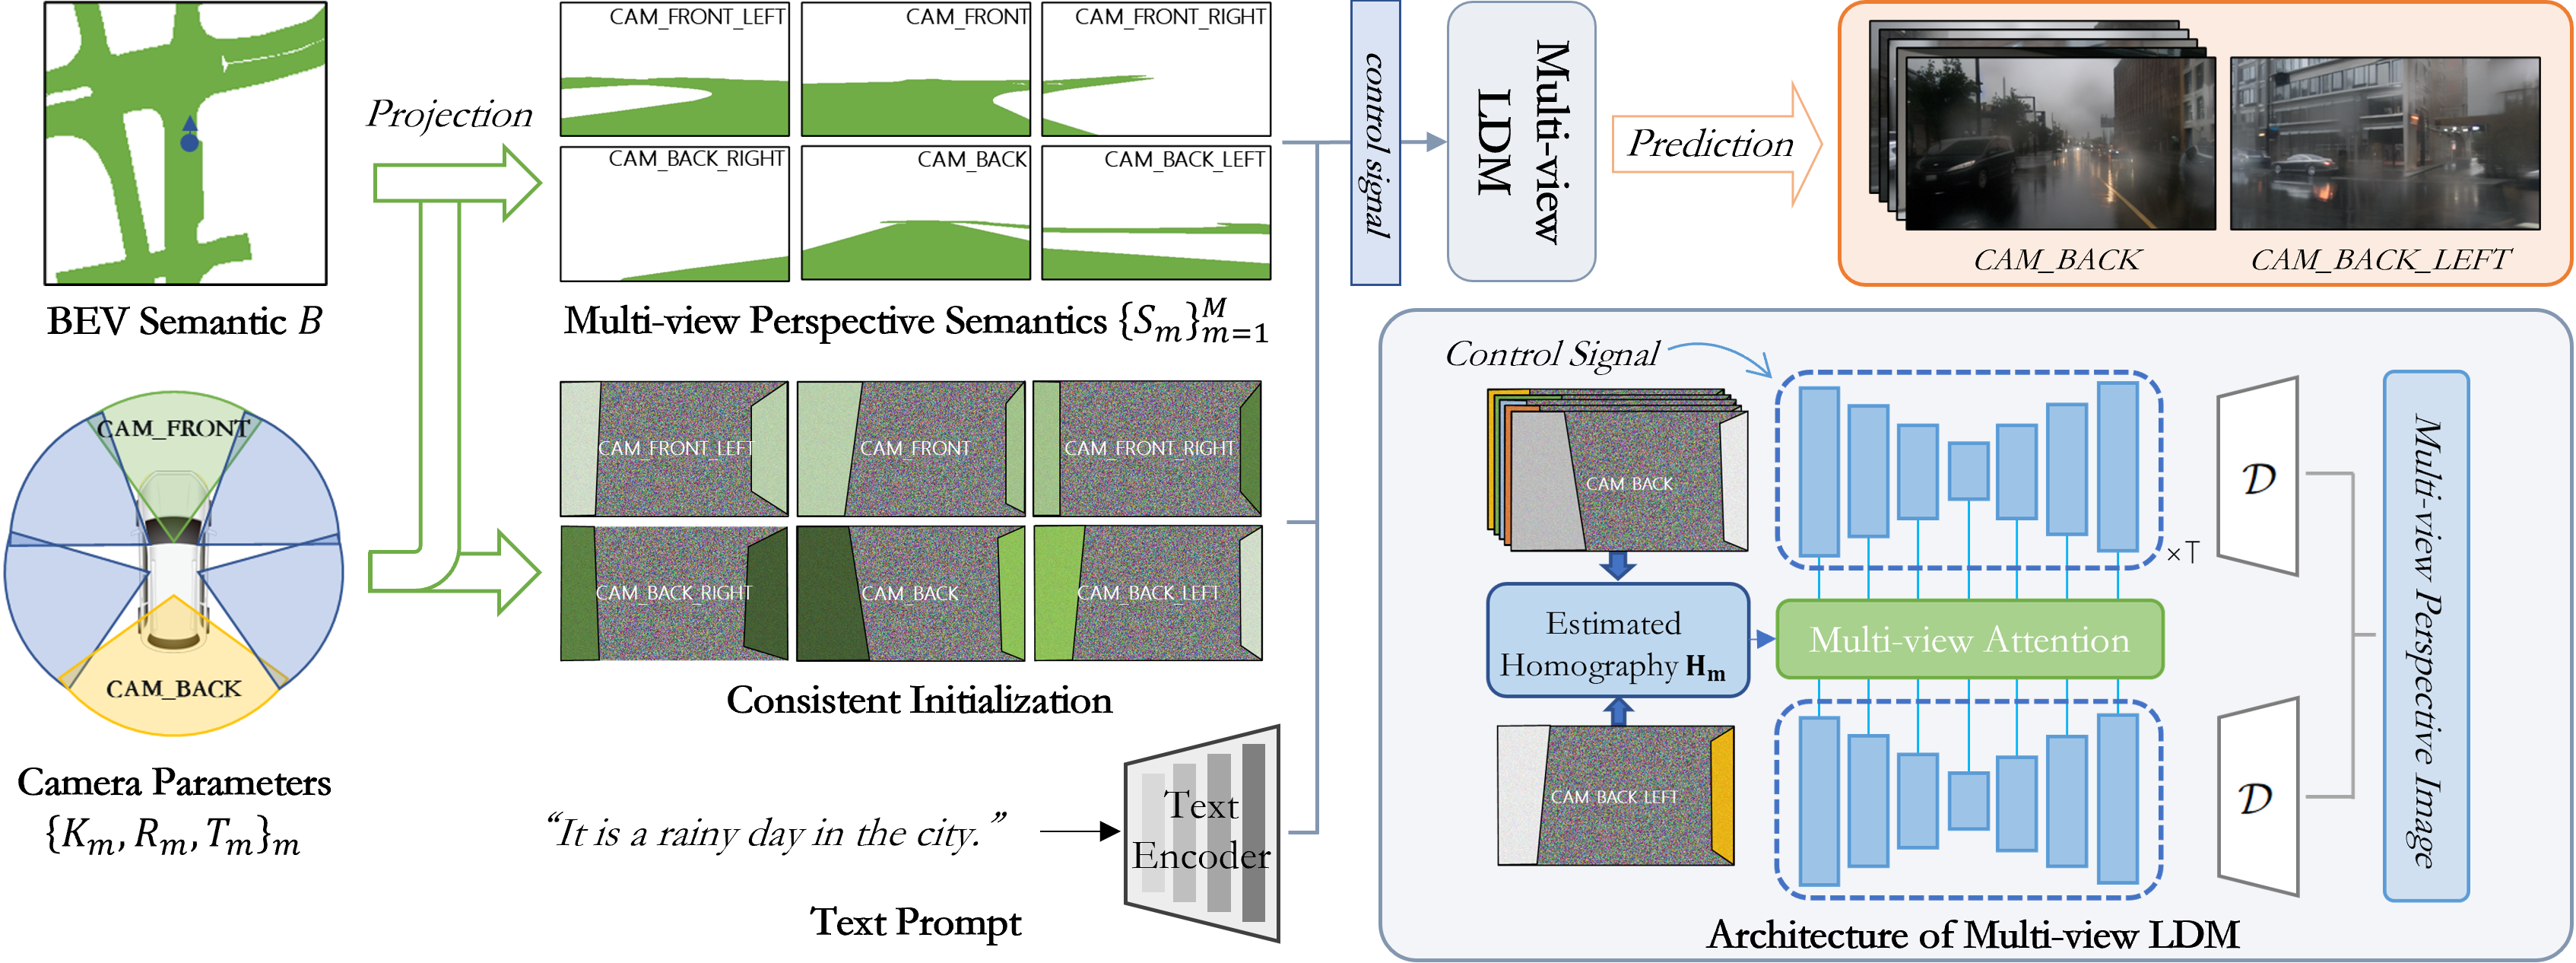
\includegraphics[width=0.95\linewidth]{figures/main.png}
\caption{MVPbev consists of two stages. The first stage projects BEV semantics to perspective view with camera parameters to maintain global semantic consistency. The second stage parses both perspective semantics and text prompts, and generates multi-view images with both visual consistency and test-time instance-level control by explicit enforcing in latent.
}
\label{fig:main}
\end{figure*}

Image editing~\cite{imageedit} and generation~\cite{rombach2021highresolution} are heated topics in computer vision. Though this can be related to a vast literature, we would focus on two lines of work, conditional image generation and novel view image synthesis, as they are closely relevant.

\noindent{\textbf{Conditional image generation}} Generative models, e.g., Gaussian Mixture model~\cite{rasmussen1999infinite} and Bayesian network~\cite{Jensen2001Bayesian}, have been a long-term research problem in machine learning and computer vision as it is able to explain complex data distribution. In particular, generative models of images are not only of great importance for unsupervised feature learning, but also enable applications such as image editing~\cite{imageedit,kawar2023imagic}. With the rise of deep learning techniques, such as auto-regressive models~\cite{chan2005probabilistic}, variational autoencoders (VAEs)~\cite{kingma2013auto}, and generative adversarial networks (GANs)~\cite{goodfellow2020generative}, as well as the emerging of huge amount of data~\cite{imagenet}, we observe photorealistic images with very good quality. Among them, conditional GANs have been well explored where various constraints, including discrete labels, text, and images, are considered. More recently, stable diffusion models~\cite{rombach2021highresolution} are widely used to generate detailed images conditioned on text descriptions. Compared to the prior art, they not only demonstrate SOTA image generation quality, but also showcase great generalizability with the help of foundation models~\cite{li2023blip}. Later on, Controlnet~\cite{zhang2023adding} largely improves the overall performance of diffusion models without losing the original robustness by allowing a diverse set of conditional controls, e.g., depth, semantics, or sketches. Despite impressive progress, multi-view or cross-view text-to-image generation still confronts issues of computational efficiency and consistency across views. To this end, MVDiffusion~\cite{Tang2023mvdiffusion} proposes a novel correspondence-aware attention module to create multi-view images from text with the ability to maintain global correspondence. Though providing good multi-view RGB images, MVDiffusion fails to generalize to more dramatic viewpoint changes or smaller overlapping areas. Perhaps the co-current work, including BEVGen~\cite{swerdlow2023street}, BEVControl~\cite{yang2023bevcontrol}, and MagicDrive~\cite{gao2023magicdrive},  are the closest to ours. The first one generates multi-view visual consistent images based on the BEV semantics by employing an auto-regressive transformer with cross-view attention. While the last two work with image sketches/semantics and text, and utilizes cross-view cross-object attention to focus more on consistency on individual contents. However, none of existing work allows test-time generalizability, e.g., view-point changes or detailed instance-level text prompts. Nor do they conduct human analysis on image generation quality. In contrast, we propose to exploit both global and local consistency to leverage semantic and visual coherency, together with our training-free objects control method to enforce detailed instance-level control. Moreover, we provide comprehensive human analysis to demonstrate the effectiveness of our method in a more reliable manner. 

% detailed human analysis are missing. In this work, we propose to exploit both global and local consistency to leverage semantic and visual coherency. In the meantime, we extend NuScenes with text prompts and conduct comprehensive human analysis to demonstrate the effectiveness of our method. 
%Perhaps the co-current work, specifically the BEVGen~\cite{?} and BEVControl~\cite{?}, are the closest to ours. The former generates multi-view visual consistent images based on the BEV semantics by employing an auto-regressive transformer with cross-view attention. In contrast, the latter works with image sketches and text, and utilizes cross-view cross-object attention to focus more on consistency on individual contents. 
% Though providing good multi-view RGB images, there are two main drawbacks of the above-mentioned methods. Firstly, they fail to enforce the visual consistency at overlapping FOVs, especially for the background. Secondly, an evaluation of the method's robustness and
% detailed human analysis are missing. In this work, we propose to exploit both global and local consistency to leverage semantic and visual coherency. In the meantime, we extend NuScenes with text prompts and conduct comprehensive human analysis to demonstrate the effectiveness of our method. 

\noindent{\textbf{Novel view image synthesis}} There are two broad categories in which the novel view synthesis methods can be divided into geometry-based and learning-based approaches. The former tries to first estimate (or fake) the approximate underlying 3D structures, followed by applying some transformation to the pixels in the input image to produce the output~\cite{avidan1997novel,zhou2016view}. The latter, on the other hand, argues that novel view synthesis is fundamentally a learning problem, because otherwise it is woefully under-constrained. More recently, neural radiance fields (NeRF)~\cite{mildenhall2021nerf}, which belong to the second category, have shown impressive performance on novel view synthesis of a specific scene by implicitly encoding volumetric density and color through a neural network. Starting from small-scales~\cite{mildenhall2021nerf}, scene-level NeRFs, such as Block-NeRF~\cite{tancik2022block}, are also proposed such that important use-cases, e.g., autonomous driving~\cite{caesar2020nuscenes} and aerial surveying~\cite{kaiser2017learning} are enabled by reconstructing large-scale environments. In contrast, our method takes the input as BEV semantics and text description and outputs multi-view perspective RGB. 
%, allowing more generalizability over modality and view-point changes. % and fine-grained control.
% Our method not only allows more controllability, but also enforces cross-view consistency both visually and semantically.